\documentclass{standalone}
% Font
\usepackage{mathpazo}
\usepackage{libertine}
\renewcommand*\sfdefault{phv}

\usepackage{tikz}
\usetikzlibrary{shapes,arrows,positioning,calc}
\tikzstyle{every node}=[font=\sffamily]
\tikzstyle{node} = [rectangle, very thick, text centered, draw=none]
\tikzstyle{arrow} = [->,thick]
\tikzstyle{line} = [thick]

\begin{document}
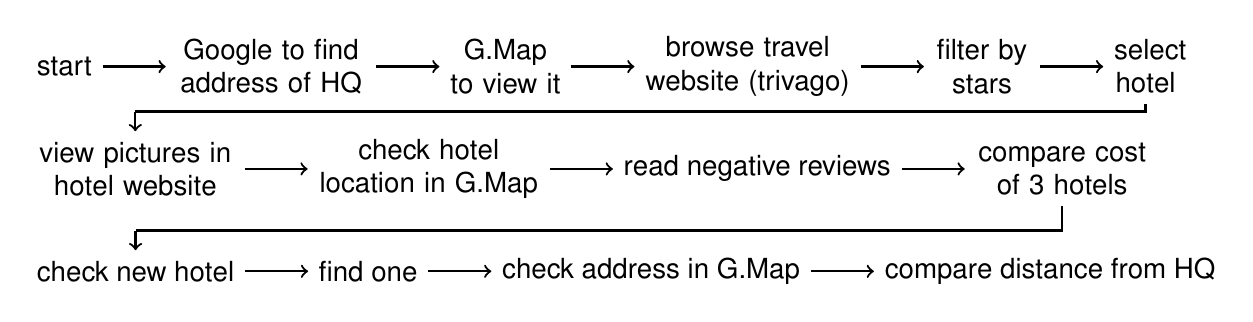
\begin{tikzpicture}[node distance=0.8cm]
\node (p0) [node] {start};
\node (p1) [node, right=of p0, text width = 2.4cm] {Google to find address of HQ};
\draw [arrow] (p0)--(p1);
\node (p2) [node, right=of p1, text width = 1.4cm] {G.Map to view it};
\draw [arrow] (p1)--(p2);
\node (p3) [node, right=of p2, text width = 2.6cm] {browse travel website (trivago)};
\draw [arrow] (p2)--(p3);
\node (p4) [node, right=of p3, text width = 1.2cm] {filter by stars};
\draw [arrow] (p3)--(p4);
\node (p5) [node, right=of p4, text width = .8cm] {select hotel};
\draw [arrow] (p4)--(p5);
\node (p6) [node, below=1.3cm of p0.west, anchor=west, text width = 2.5cm] {view pictures in hotel website};
\draw [line] (p5)|-($(p6.north) + (0,.25cm)$);
\draw [arrow] ($(p6.north) + (0,.25cm)$) -- (p6);
\node (p7) [node, right=of p6, text width = 2.8cm] {check hotel location in G.Map};
\draw [arrow] (p6)--(p7);
\node (p8) [node, right=of p7] {read negative reviews};
\draw [arrow] (p7)--(p8);
\node (p9) [node, right=of p8, text width =2.2cm] {compare cost of 3 hotels};
\draw [arrow] (p8)--(p9);
\node (p10) [node, , below=1.3cm of p6.west, anchor=west] {check new hotel};
\draw [line] (p9)|-($(p10.north) + (0,.25cm)$);
\draw [arrow] ($(p10.north) + (0,.25cm)$) -- (p10);
\node (p11) [node, right=of p10] {find one};
\draw [arrow] (p10)--(p11);
\node (p12) [node, right=of p11] {check address in G.Map};
\draw [arrow] (p11)--(p12);
\node (p13) [node, right=of p12] {compare distance from HQ};
\draw [arrow] (p12)--(p13);

%\draw [line] (p7)|-($(p8.north) + (0,.25cm)$);
%\draw [arrow] ($(p8.north) + (0,.25cm)$) -- (p8);

\end{tikzpicture} 

\end{document}